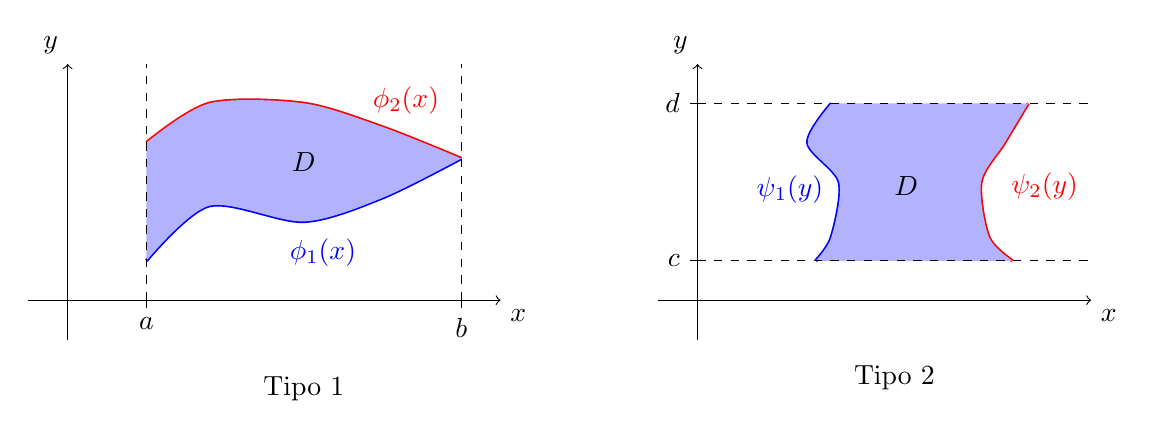
\begin{tikzpicture}
    % parámetros
    \def\a{0}    % a
    \def\b{4}    % b
    \def\c{0.5}    % c
    \def\d{2.5}  % d
  
    %—————— Región tipo I ——————————————————————————————————————————————————
    \begin{scope}
      % ejes
      \draw[->] (\a-1.5,0) -- (\b+0.5,0) node[below right] {$x$};
      \draw[->] (-1,-0.5) -- (-1,\d+0.5)    node[above left]  {$y$};
      % curvas phi1 y phi2
      \draw[red,   very thick, smooth] plot coordinates {
        (\a,2) (0.8,2.5) (2,2.5) (3,2.2) (\b,1.8)
      } node[above=2pt, xshift=-20pt, yshift=10pt] {$\phi_2(x)$};
      \draw[blue,  very thick, smooth] plot coordinates {
        (\a,0.5) (0.8,1.2) (2,1) (3,1.3) (\b,1.8)
      } node[below, xshift=-50pt, yshift=-25pt] {$\phi_1(x)$};
      % relleno de la región entre curvas
      \begin{scope}
        \clip plot[smooth] coordinates {
          (\a,2) (0.8,2.5) (2,2.5) (3,2.2) (\b,1.8)
        }
        -- plot[smooth] coordinates {
          (\b,1.8) (3,1.3) (2,1) (0.8,1.2) (\a,0.5)
        } -- cycle;
        \fill[blue!30] (\a-0.5,-0.5) rectangle (\b+0.5,\d+0.5);
      \end{scope}
      % líneas punteadas en x=a, x=b y sus etiquetas
      \draw[dashed] (\a,0) -- (\a,\d+0.5);
      \draw (\a, 0) -- ++(0,-0.1) node[below] {$a$};
      \draw[dashed] (\b,0) -- (\b,\d+0.5);
      \draw (\b, 0) -- ++(0,-0.1) node[below] {$b$};
      % título
      \node[below,yshift=-10pt] at ({(\a+\b)/2},-0.5)
        {Tipo 1};
      \node[below] at ({(\a+\b)/2},2) {$D$};
    \end{scope}
  
    %—————— Región tipo II —————————————————————————————————————————————————
    \begin{scope}[xshift=7cm]
      % ejes
      \draw[->] (-0.5,0) -- (\b+1,0)   node[below right] {$x$};
      \draw[->] (0,-0.5) -- (0,\d+0.5) node[above left]  {$y$};
      % curvas psi1 y psi2
      \draw[blue, very thick, smooth] plot coordinates {
        (1.5,\c) (1.7,0.8) (1.8,1.5) (1.4,2) (1.7,\d)
      } node[above left, xshift=1pt, yshift=-40pt] {$\psi_1(y)$};
      \draw[red,  very thick, smooth] plot coordinates {
        (4,\c) (3.7,0.8) (3.6,1.5) (3.9,2) (4.2,\d)
      } node[right, xshift=-10pt, yshift=-30pt]{$\psi_2(y)$};
      % relleno de la región
      \begin{scope}
        \clip plot[smooth] coordinates {
            (1.5,\c) (1.7,0.8) (1.8,1.5) (1.4,2) (1.7,\d)
            }
        -- plot[smooth] coordinates {
          (4.2,\d) (3.9,2) (3.6,1.5) (3.7,0.8) (4,\c)
        } -- cycle;
        \fill[blue!30] (-0.5,\c-0.5) rectangle (\b+1,\d+0.5);
      \end{scope}
      % líneas punteadas en y=c, y=d y sus etiquetas
      \draw[dashed] (0,\c) -- (\b+1,\c);
      \draw (0, \c) -- ++(-0.1,0) node[left] {$c$};
      \draw[dashed] (0,\d) -- (\b+1,\d);
      \draw (0, \d) -- ++(-0.1,0) node[left] {$d$};
      % título
      \node[below,yshift=-20pt] at ({(\b+1)/2},\c-0.5)
        {Tipo 2};
        \node[below] at ({(\b+1.3)/2},\c+1.2) {$D$};
    \end{scope}
  
  \end{tikzpicture}